\section{Shared Entities using Generics}\label{sec:shared_entities}

A \emph{shared entity} is a concept that often arises in blockchain
applications. Namely, a shared entity is something divided into \emph{shares}. Participants,
that hold shares, are called \emph{shareholders} and can dynamically
sell and buy shares. An example of a shared entity is a corporation,
where shares represent units of possess of the company. Another example is
a voting community, where shares represent the voting power of each given voter.
A further example is the set of the validator nodes of a proof of stake blockchain,
where shares represent their voting power and remuneration percentage.

\begin{figure}[ht]
  \begin{center}
    \begin{lstlisting}[language=Takamaka]
public interface SharedEntity
      <S extends PayableContract, O extends Offer<S>>
      extends SharedEntityView<S> {

  @View StorageSetView<O> getOffers();

  @View BigInteger sharesOnSaleOf(S shareholder);

  @FromContract(PayableContract.class) @Payable
  void place(BigInteger ticket, O offer);

  @FromContract(PayableContract.class) @Payable
  void accept(BigInteger ticket, S buyer, O offer);

  class Offer<S extends PayableContract> extends Storage {
    public final S seller;
    public final BigInteger sharesOnSale;
    public final BigInteger cost;
    public final long expiration;

    public Offer(S seller, BigInteger sharesOnSale, 
                 BigInteger cost,long duration) {
      this.seller = seller;
      this.sharesOnSale = sharesOnSale;
      this.cost = cost;
      this.expiration = now() + duration;
    }

    @View public boolean isOngoing() {
      return now() <= expiration;
    }
  }
}
    \end{lstlisting}
  \end{center}
  \caption{A simplified part of our shared entity interface.}\label{fig:shared_entity}
\end{figure}

In general, two concepts are specific to each implementation of shared entities:
who are the potential shareholders and how offers for selling shares work.
Therefore, one can parameterize the interface of a shared entity with two type variables:
\<S> is the type of the shareholders and \<O> is the type of the sale offers of shares.

The \<SharedEntityView> interface at the top of the hierarchy in Fig.~\ref{fig:hierarchy-entities}
defines the read-only operations on a shared entity. This view is \emph{static}, in the sense that it
does not specify the operations for transfers of shares. Therefore, its only type parameter is \<S>:
any contract can play the role of the type for the shareholders of the entity.
Method \<getShares> yields a snapshot of the
current shares of the entity (who owns how much). Method \<getShareholders> yields the shareholders.
It is not \<@View>, since it creates a new stream, which is a side-effect.
Method \<isShareholder> checks if an object is a shareholder. Method \<sharesOf> yields
the number of shares of a shareholder. As typical in Takamaka, a \<snapshot> method allows one
to create a frozen read-only copy of an entity (in constant time), useful when an entity must be queried from
a client without the risk of race conditions if another client is modifying the same entity concurrently.

The \<SharedEntity> subinterface adds methods for transfer of shares
(see Fig.~\ref{fig:shared_entity}).
It includes an inner class \<Offer> that models sale offers:
it specifies who is the seller of the shares,
how many shares are being sold, the requested price and the expiration of the offer.
Method \<isOngoing> checks if an offer has not expired yet.
Implementations can subclass \<Offer> if they need more specific offers.
Offers can be placed on sale
by calling the \<place> method with a sale \<offer>
(see Fig.~\ref{figure.shared_entity}).
This method is annotated as \<@FromContract> since the caller must be
identified (or otherwise anybody could sell the shares of anybody else) and
as \<@Payable> so that implementations can require
to pay a \<ticket> to place shares on sale.
The sale offer is passed as a parameter to \<place>, hence it must have been created before calling that method.
The set of all sale offers is available through \<getOffers>. Method \<sharesOnSale> yields the
cumulative number of shares on sale for a given shareholder.
Who wants to buy shares calls method \<accept> with the accepted \<offer>
and with itself as \<buyer> (the reason will be explained soon)
and becomes a new shareholder or increases
its cumulative number of shares (if it was a shareholder already).
Also this method is \<@Payable>, since its caller must pay \<ticket> $\ge$ \<offer.cost>
coins to the seller.
This means that shareholders must be able to receive payments and that
is why \<S extends PayableContract>: only \<PayableContract>s are guaranteed to have a
\<receive> method in Takamaka.

\begin{figure}[ht]
\centering
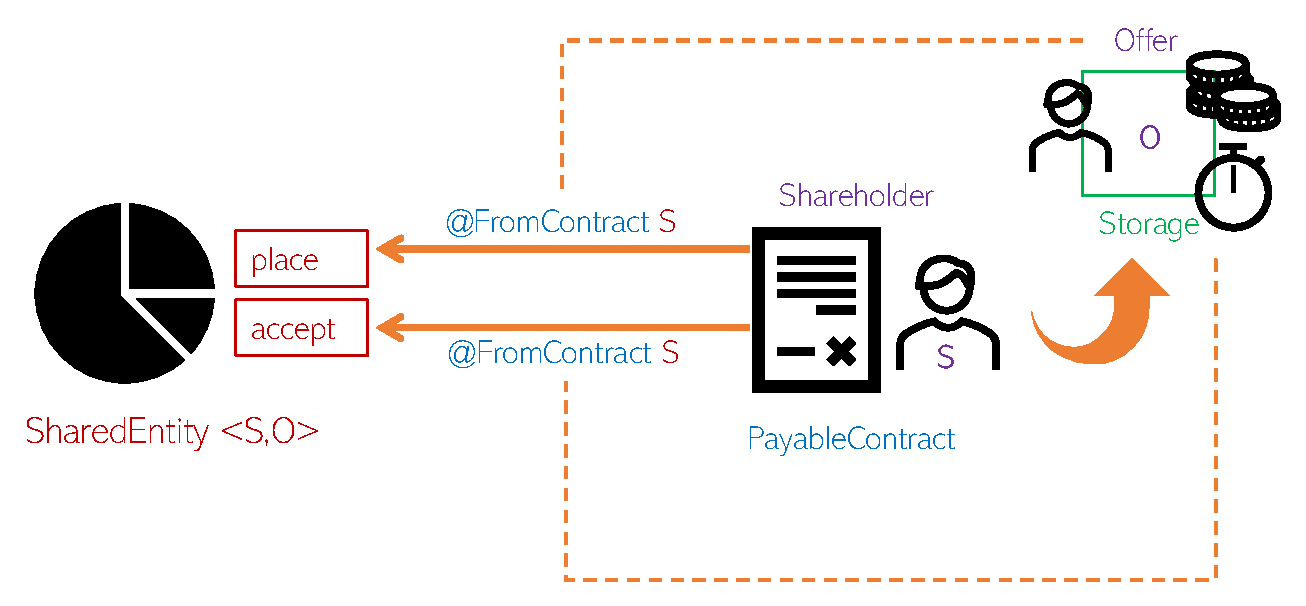
\includegraphics[width=.9\linewidth]{figures/shared_entity}
\caption{Exemplification of a Takamaka shared entity and of its connections with the objects persisted in the blockchain.}
\label{figure.shared_entity}
\end{figure}

As said before, the annotation \<@FromContract> on both \<place> and \<accept> enforces that only
contracts can call these methods.
These callers must be (old or new) shareholders,
hence they must have type \<S>. Therefore, one would like to write
\<@FromContract(S.class)>. Unfortunately, Java does not allow a generic type variable \<S>
in the syntax \<S.class>. Due to this syntactical limitation of Java,
the best we could write in Fig.~\ref{fig:shared_entity} is \<@FromContract(PayableContract.class)>,
which allows \emph{any} \<PayableContract> to call these methods, not just those of type \<S>.
Since the syntax of the language does not support our abstraction, we will have to
program explicit dynamic checks in code, as shown later, and this will be the reason of the
parameter \<buyer> in \<accept>.



\begin{figure}[tp]
  \begin{center}
    \begin{lstlisting}[language=Takamaka]
public class SimpleSharedEntity
    <S extends PayableContract,O extends Offer<S>>
    extends PayableContract implements SharedEntity<S,O> {

  private StorageTreeMap<S,BigInteger> shares = new StorageTreeMap<>();
  private StorageSet<O> offers = new StorageTreeSet<>();

  public SimpleSharedEntity(S shareholder, BigInteger share) {
    addShares(shareholder, share);
  }

  @Override @View public final BigInteger sharesOf(S shareholder) {
    return shares.getOrDefault(shareholder, ZERO);
  }

  @Override @FromContract(PayableContract.class) @Payable
  public void place(BigInteger amount, O offer) {
    require(offer.seller == caller(), "unauthorized");
    require(shares.containsKey(offer.seller), "unauthor.");
    require(sharesOf(offer.seller) - sharesOnSaleOf(offer.seller) >= 
            offer.sharesOnSale, "not enough shares");
    offers.add(offer);
  }

  @Override @FromContract(PayableContract.class) @Payable
  public void accept(BigInteger amount, S buyer, O offer) {
    require(caller() == buyer, "unauthorized");
    require(offers.contains(offer), "unknown offer");
    require(offer.isOngoing(), "the offer is not ongoing");
    require(offer.cost <= amount, "not enough money");
    offers.remove(offer);
    removeShares(offer.seller, offer.sharesOnSale);
    addShares(buyer, offer.sharesOnSale);
    offer.seller.receive(offer.cost);
  }

  @Override @View public final BigInteger sharesOnSaleOf(S shareholder) {
    return offers.stream()
      .filter(o -> o.seller == shareholder && o.isOngoing())
      .map(offer -> offer.sharesOnSale)
      .reduce(ZERO, BigInteger::add);
  }
}
    \end{lstlisting}
  \end{center}
  \caption{A simplified part of our implementation of the shared entity interface.}\label{fig:simple_shared_entity}
\end{figure}

Fig.~\ref{fig:simple_shared_entity} shows a portion of our \<SimpleSharedEntity>
implementation of the \<SharedEntity> interface in Fig.~\ref{fig:shared_entity}, that
uses two fields: \<shares> maps each shareholder to the amount of shares the it holds and
\<offers> collects the offers that have been placed.
The constructor initially populates the map \<shares> with the initial shareholder.
Other shareholders can be added later, by buying shares\footnote{In the real code, the class has
  constructors to create shared entities with a \emph{set} of initial shareholders. This paper
  reports a simplification of the actual code.}.
Method \<sharesOf> simply accesses
\<shares>, by using zero as default. Method \<place> requires its \<caller()> to be
the seller identified in the \<offer>. This forbids shareholders to sell shares on behalf of others.
Moreover, this guarantees that the caller has type \<S>, the type of \<offer.seller>.
As it has been said before, this cannot be expressed with the syntax of the language.
Method \<place> further requires the seller to be a shareholder with at least \<offer.sharesOnSale>
shares not yet placed on sale. This forbids to oversell more shares
than one owns. At the end, \<place> adds the \<offer> to the set of \<offers>.
Method \<accept> requires that who calls the method must be \<buyer>. Hence, successful
calls to \<accept> can only pass the same caller for \<buyer>. This is a trick to enforce the
caller to have type \<S>, since the syntax of the language does not allow one to express it,
as we explained before. Then \<accept> requires the \<offer> to exist, to be still ongoing
and to cost no more than the \<amount> of money provided to \<accept>. If that is the case,
the \<offer> is removed from the \<offers>, shares are moved from seller to buyer (code not
shown in Fig.~\ref{fig:simple_shared_entity}) and the seller of the \<offer>
receives the required price \<offer.cost>.
